\section{Experiment 1: Basic HIGHLIGHTS}
Experiment 1 compared summaries generated by the basic HIGHLIGHTS algorithm, which only considers state importance, with summaries generated with the \emph{Random} and \emph{First} baselines. 40 participants were recruited through Amazon Mechanical Turk (23 female, Mean age = 35.35, STD = 10.4).  


%\label{sec:exp1res}
\paragraph{Agent Selection Results}
\label{sec:exp1res}
As shown in Figure~\ref{fig:highlightsRes}, participants were more likely to choose the better performing agents when shown summaries generated by the HIGHLIGHTS algorithm compared to the baselines. The analysis shows statistically significant and substantial differences in performance when comparing HIGHLIGHTS to  \emph{First} ($\chi^2=49.79, p<1^{-10}, OR = 12.09$) and when comparing HIGHLIGHTS to \emph{Random} ($\chi^2=6.93, p=0.001, OR = 2.38$). 

When comparing HIGHLIGHTS and \emph{First}, we found a  significant difference for all three agent comparison types (low, medium and high difficulty). When comparing HIGHLIGHTS to \emph{Random}, we observed a significant difference only for the \emph{medium-difficulty} comparison (\emph{400E} vs. \emph{2000E} agents). This makes sense as the difference between the \emph{200E} and \emph{400E} agents is relatively small, making the comparison hard with any summary. The difference between the \emph{200E} vs. \emph{2000E} agents is very substantial, making it easier to identify the better agent even with random trajectories. Interestingly, for the low-difficulty comparison, the summaries generated by \emph{First} were particularly misleading. We hypothesize the reason for this is that participants saw the \emph{2000E} agent taking more risks initially, as participants' explanations often referred to the \emph{2000E} agent behavior as risky, e.g. ``Player B [2000E] made some risky turns which will end his play before Player A [200E].'' 

We observed different types of explanations provided by participants. Some explanations referred directly to the capabilities demonstrated by the agent in the summary, e.g. ``B [2000E] seems like they are better at actually eating the ghosts''. Other participants noted the state of the board shown in different summaries, e.g. ``B has more of the screen cleared''. Some explanations described the general behavior of the agent, e.g. ``Pacman B seems to be effective at routing'' or how Pacman's strategy compares to their own strategy, e.g. ``He went the way I would have.'' Last, some explanations referred to specific events, e.g. ``Pacman a looked like it was about to be cornered.'' 

The type of explanation provided often depended on the summary method used and the difficulty of the agent comparison. Participants' explanations when shown HIGHLIGHTS summaries for the low-difficulty and medium-difficulty comparisons typically referred to specific capabilities they observed, e.g. ``Player A [2000E] is eating ghost so earning more points.'' We observed fewer such explanations for the high-difficulty comparison, e.g. ``Player B has eaten one power pill which means he's had the chance to go after the ghosts (for more points) at least once.  Also seems to have eaten more dots on the whole than Player A.'' Explanations for this comparison more often pointed to the state of the board or provided a general impression of the agent's behavior.
%Other explanations referred to the state of the board shown in the trajectories, e.g. ``B has more of the screen cleared'', or provided a general impression of the agent's behavior, e.g. ``Pacman B seems to be effective at routing''. 
For the \emph{First} summaries, participants typically conveyed their general impression of the agent's behavior. Explanations for the \emph{Random} baseline were similar to those given in the HIGHLIGHTS condition for the low-difficulty comparison, but tended to refer to more general agent behaviors for the medium- and high-difficulty comparisons (the analysis of these summaries is more difficult as each participant could observe a different \emph{Random} summary).

\begin{figure}[h]
	%\centering
	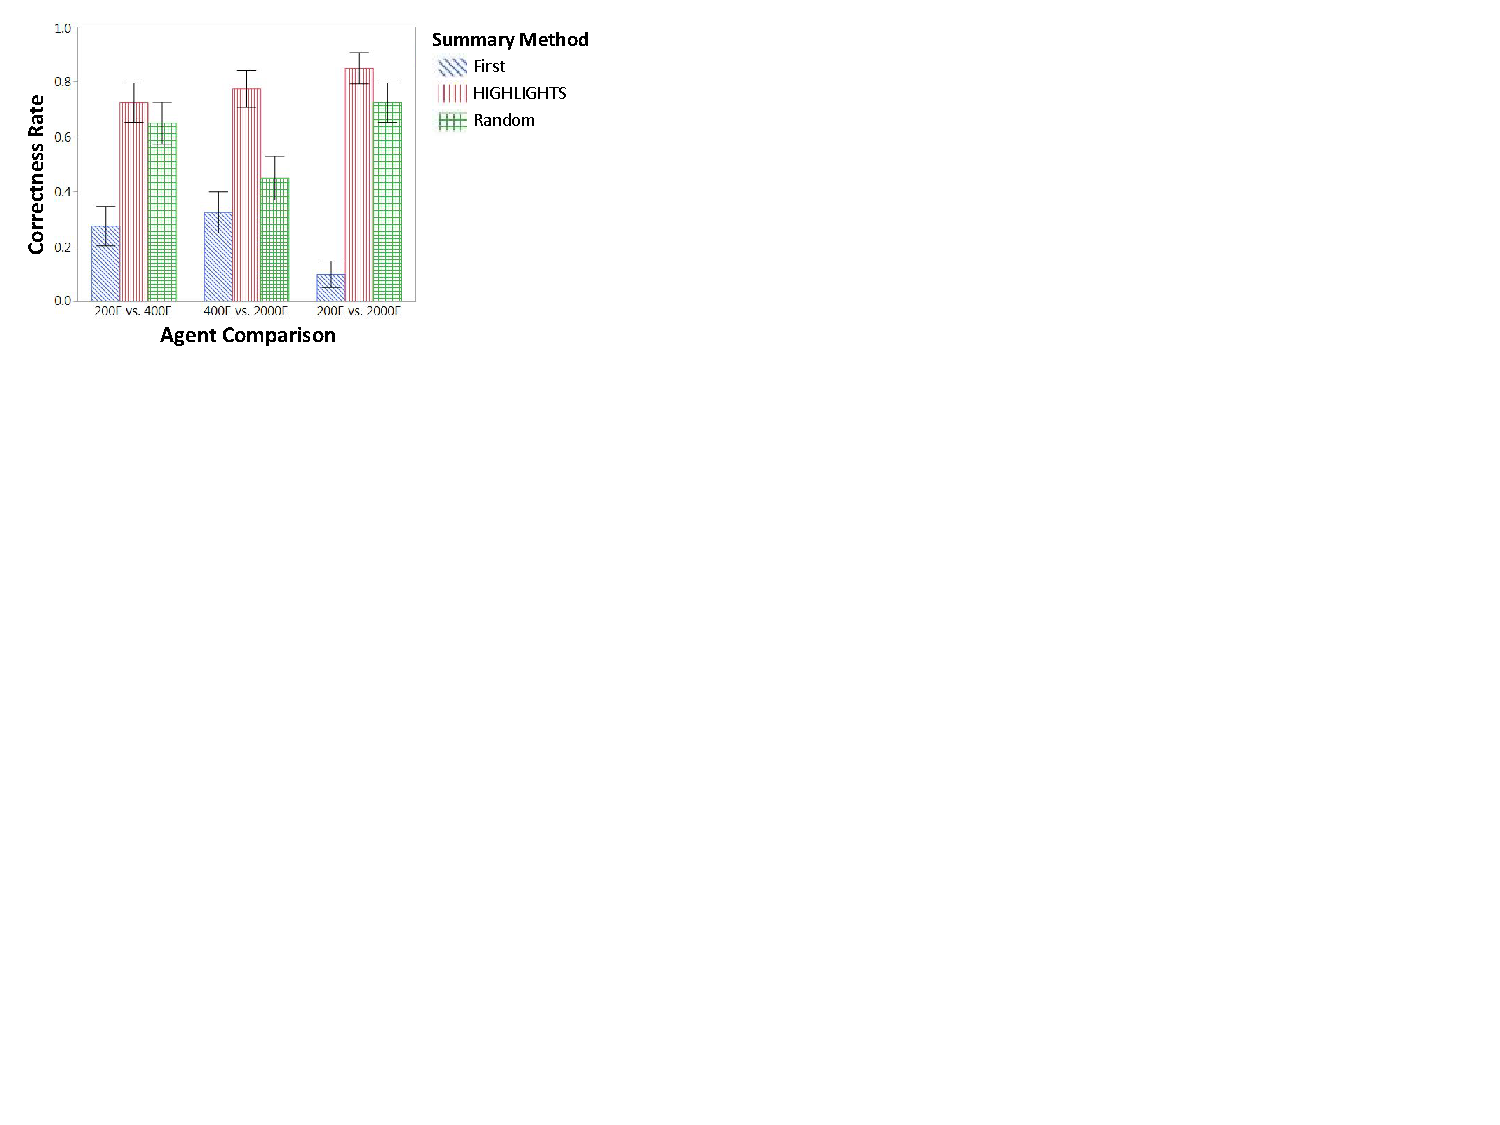
\includegraphics[width=0.9\columnwidth]{figs/correctnessExp1figForPaper.pdf}\\
	\caption{Correctness rate of participants in the agent selection task (Experiment 1).}
	\label{fig:highlightsRes}
	\vspace{-0.3cm}
\end{figure}

Figure~\ref{fig:highlightsConf} shows the distribution of participants' confidence ratings when choosing an agent to play on their behalf. Participants were more confident in their choice of agents when presented with HIGHLIGHTS summaries than they were when presented with summaries generated by \emph{First}. The differences were significant for the medium-difficulty ($\chi^2=22.04, p<0.001, OR = 7.44$) and low-difficulty ($\chi^2=13.84, p<0.001, OR = 3.64$) comparisons. We observed mixed results when comparing participants' confidence when reviewing HIGHLIGHTS and \emph{Random} summaries. When presented with the low-difficulty comparison, participants were significantly more confident when shown \emph{Random} summaries ($\chi^2=6.96, p=0.008, OR = 2.214$)
%, although they performed objectively worse with \emph{Random} summaries, on average (though this difference was not statistically significant). 
When making the low-difficulty comparisons, participants were significantly more confident with HIGHLIGHTS summaries ($\chi^2=5.819, p=0.016, OR = 2.3$). Interestingly, we found no difference in confidence for the medium-difficulty comparison, although participants performed significantly better with HIGHLIGHTS summaries in this agent comparison task. This suggests that people's confidence might not correlate with their actual ability to assess agents' capabilities. We hypothesize that a reason for this is that they only get to review a short summary, and they might think it was sufficient because they are unaware of the information that was \emph{not} included in the summary.
%We also note that as can be seen in Figure~\ref{fig:highlightsConf}, there was much lower variance in participants' confidence ratings for the HIGHLIGHTS summaries compared to the variance in ratings for the two baseline summaries. 



\begin{figure}[h]
	%\centering
	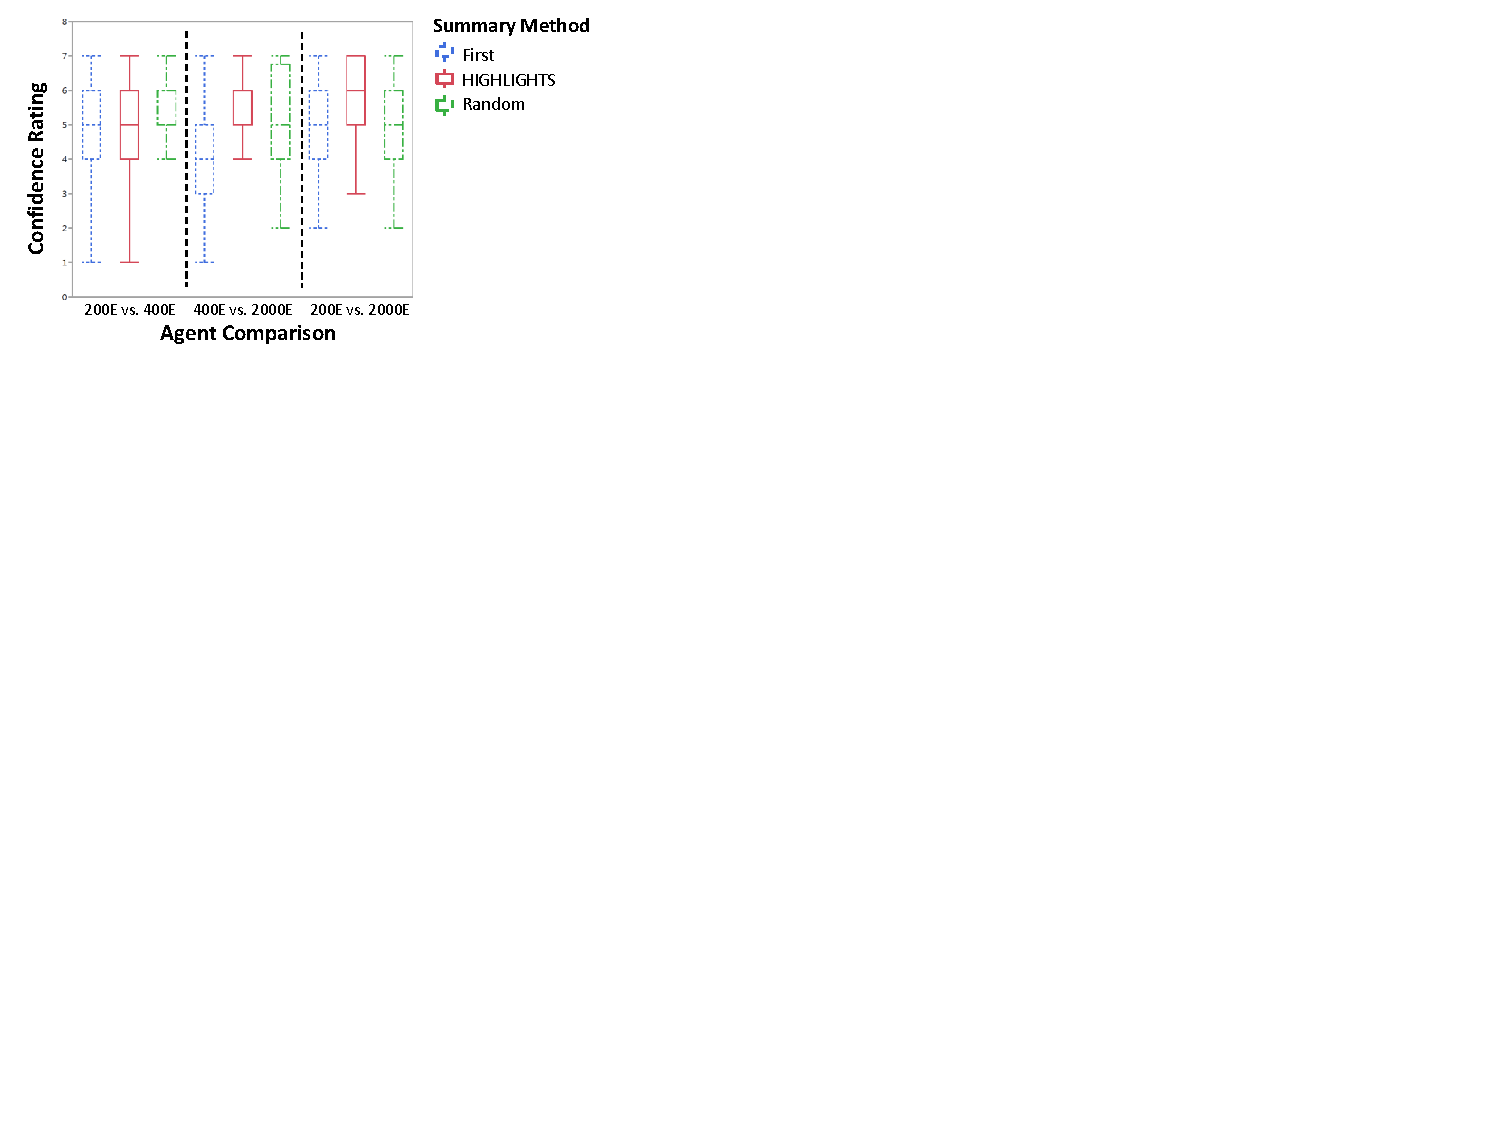
\includegraphics[width=0.89\columnwidth]{figs/confidenceExp1figForPaper.pdf}\\
	\caption{Participants' confidence rating on a scale of 1--7 when selecting an agent (Experiment 1).}
	\label{fig:highlightsConf}
	\vspace{-0.3cm}
\end{figure}


\paragraph{Summary Preferences}
% In addition, we showed participants with pairs of video summaries of \emph{the same} agent, generated by \emph{different} methods and elicited their subjective preference by asking them to rate which summary was more helpful for assessing the capabilities of the agent (they were told the videos were of the same agent). The ratings were on a 1--7 Likert scale where 1 is ``summary A was more helpful'' and 7 is ``summary B was more helpful''. We normalized the scores such that scores closer to 7 suggest a preference for HIGHLIGHTS (in the experiment the assignment to summary A and B was randomized). 
The distribution of participants' subjective preferences ratings for the different summaries are shown in Figure~\ref{fig:highlightsPrefs}. Recall, that a rating closer to 7 means they stated that the summary generated by HIGHLIGHTS was more helpful in assessing the agent's capability, while a rating closer to 1 indicates that they found the other summary (generated by either \emph{First} or \emph{Random}) as more helpful. That is, ratings greater than 4 indicate a preference for HIGHLIGHTS. The ratings are shown separately for each type of agent for which summaries were presented. 

\begin{figure}[h]
	%\centering
	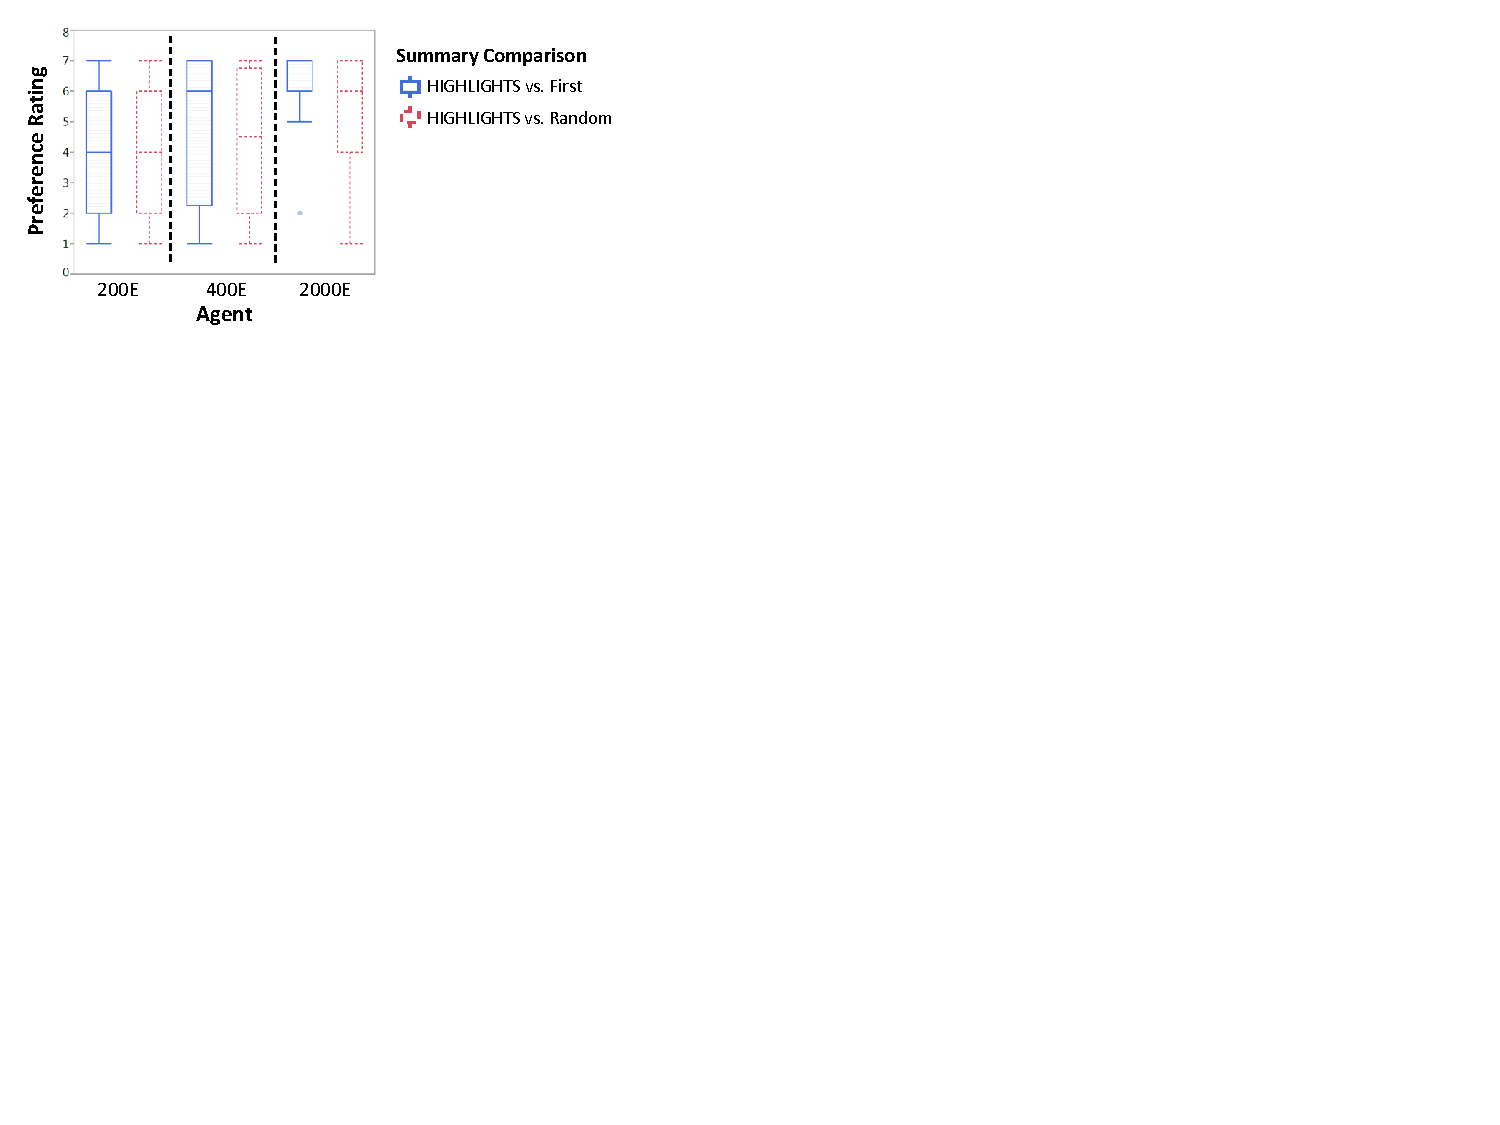
\includegraphics[width=0.85\columnwidth]{figs/preferencesExp1figForPaper.pdf}\\
	\caption{Participants' preference rating on a scale of 1--7, where 7 = ``HIGHLIGHTS is more helpful'' (Experiment 1).}
	\label{fig:highlightsPrefs}
	\vspace{-0.3cm}
\end{figure}

On average, participants preferred summaries generated by HIGHLIGHTS over summaries generated by \emph{First} ($Median = 6$) and summaries generated by \emph{Random} ($Median = 5$). The only statistically significant differences in preferences were for the highest performing agent (\emph{2000E}). The ratings were significantly greater than 4 both when comparing HIGHLIGHTS with \emph{First} ($Median = 7, p<0.001$) and when comparing HIGHLIGHTS with \emph{Random} ($Median = 6, p=0.009$). We attribute this stronger preference to the greater difference between summaries generated by different methods when considering agents that have more capabilities. For example, the highest performing Pacman agent was able to both escape ghosts and eat the power pellets which let it eat ghosts. The HIGHLIGHTS summary for this agent included trajectories demonstrating this capability, while \emph{First} summaries did not show it, and only some \emph{Random} summaries did. Participants often referred to the skills demonstrated in the summary when explaining their ratings of these summaries, e.g. ``A [HIGHLIGHTS] was better for showing how good they were at leading the ghosts.'' In contrast, the lowest performing agent did not have many capabilities, and therefore there was less difference between the summaries generated by the different methods. Another possible explanation for this difference is that because the \emph{200E} and \emph{400E} agents are less trained, their Q-values are less accurate, making their judgment of state importance inferior, and thus potentially making the summaries less useful. 

%When explaining their ratings of the helpfulness of different summaries, participants often referred to the skills demonstrated in the video, e.g. ``A [HIGHLIGHTS] was better for showing how good they were at leading the ghosts'' or the state of the game shown, e.g. ``[video] A shows more of the late game''. Few explanations refereed to the diversity of the summary, e.g. ``[video] A [HIGHLIGHTS] showed more scenarios than B [\emph{First}] did''.




